\documentclass[../main.tex]{subfiles}
\begin{document}
\chapter{Resultados}
Para conseguir resultados significativos, no sólo debieron seguirse los métodos descritos en el capítulo anterior, sino que también estos se realizaron en un orden particular, que permitió determinar las condiciones de las técnicas subsecuentes además de prevenir mediciones innecesarias. En la figura \ref{fig:resdiag} se puede observar un diagrama del orden seguido.
\begin{figure}[H]
    \centering
    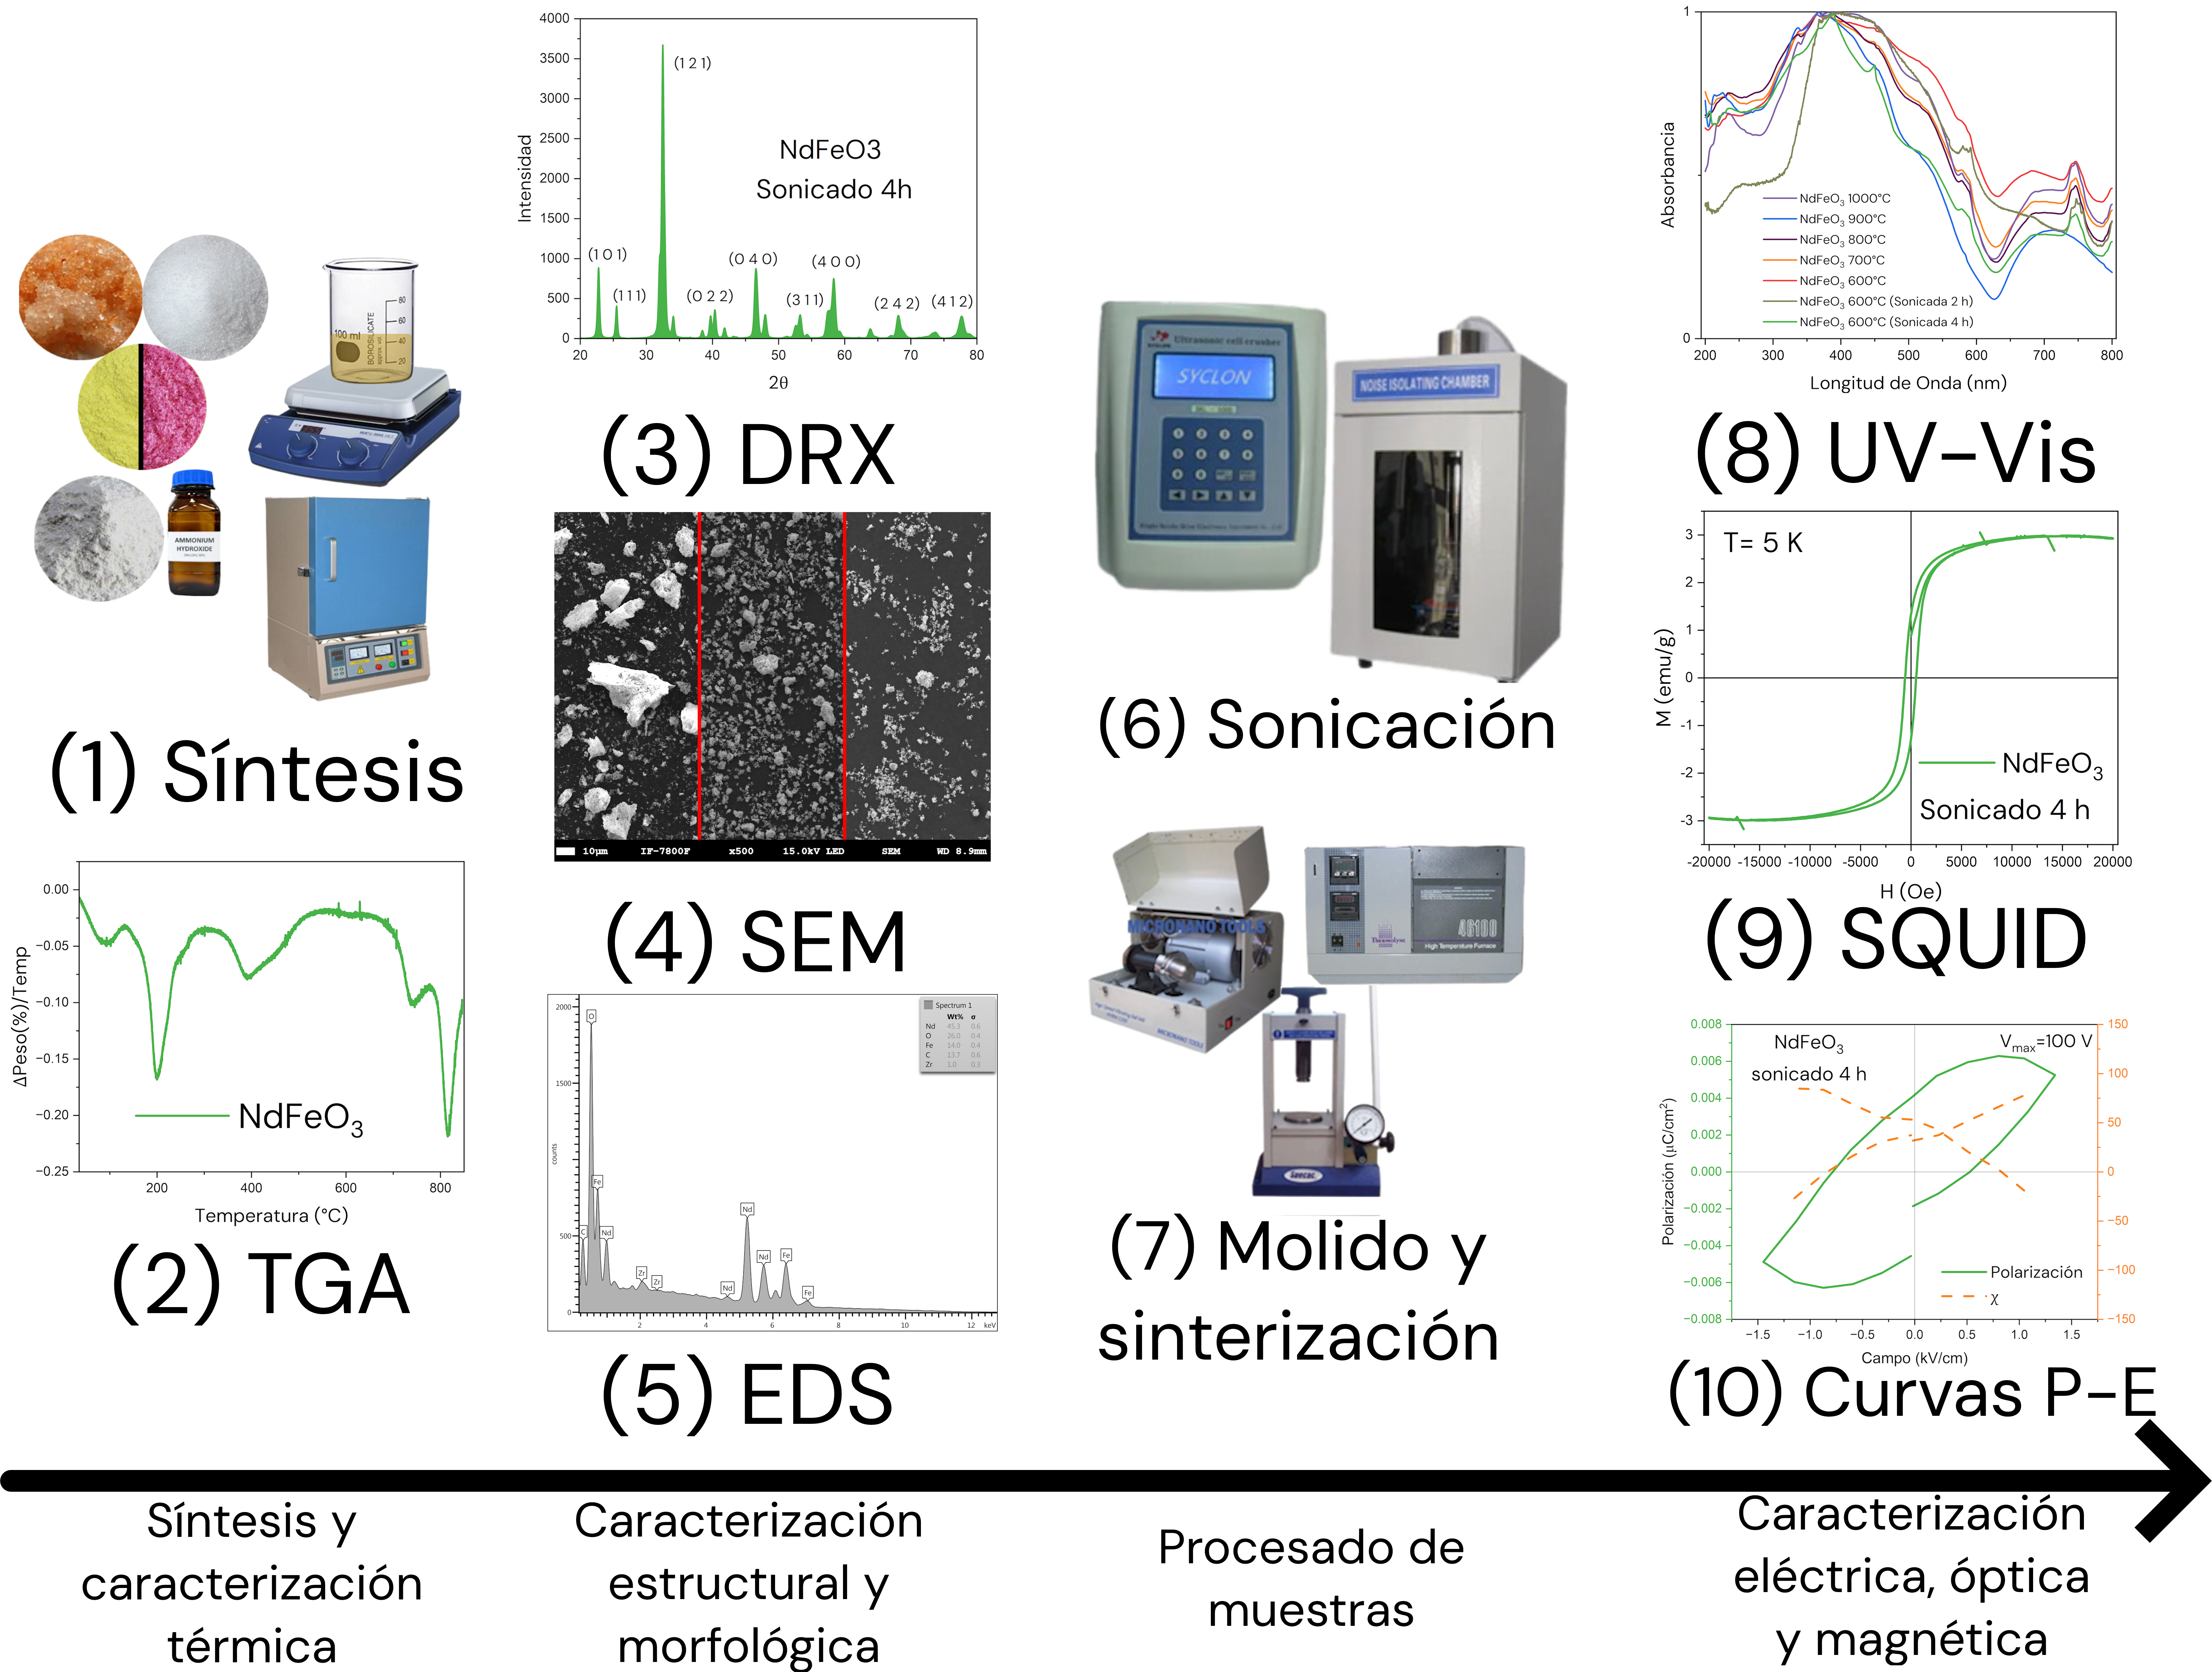
\includegraphics[width=0.7\textwidth]{fig/diagresultados.png}
    \caption{Resultados obtenidos mediante las técnicas de síntesis y caracterización descritas en el capítulo 4.}
    \label{fig:resdiag}
\end{figure}
\section{Muestras Sintetizadas} \label{sec:sintesis}
Se sintetizaron un total de 9 muestras de 1gr de \neod{} y 8 de \sama{}. Una muestra de cada ortoferrita fue reservada para realizar un análisis termogravimétrico. A través de éste, se determinó la temperatura mínima de calcinación para ambas ortoferritas, como se reporta en la sección \ref{sec:TGA}.

Con estas temperaturas en mente, 600\gradoC{} para el \neod{} y 700\gradoC{} para el \sama{}, se calcinaron el resto de muestras, 4 muestras de \neod{} se calcinaron a 600\gradoC{}, para las otras 4 se aumentó la temperatura 100\gradoC{} por cada una, es decir, se calcinaron a 700, 800, 900 y 1000\gradoC{} respectivamente.

Por otro lado, para el \sama{} se calcinaron 4 muestras a 700\gradoC{}, aumentando la temperatura de la misma forma que en el caso del \neod{} para las otras 3, es decir, se calcinaron a 800, 900 y 1000\gradoC{} respectivamente.
\section{Caracterización}
Las técnicas realizadas en esta sección pueden dividirse en tres apartados. Análisis térmico (sección \ref{sec:analisistermico}), que permite optimizar las condiciones de síntesis, análisis estructural, morfológico y de composición (sección \ref{sec:analisisestruc}), que permite comprobar la presencia de la fase que se busca y estudiar la forma física de las muestras sintetizadas y, finalmente, análisis óptico, magnético y eléctrico (sección \ref{sec:analisisoptmagelec}), con el fin de relacionar estas propiedades con las estudiadas en la sección anterior. En conjunto, estos análisis permiten una caracterización apropiada de las muestras obtenidas en función del tamaño de partícula.
\subsection{Análisis Térmico} \label{sec:analisistermico}
\subsubsection{Análisis Termogravimétrico} \label{sec:TGA}

\subsection{Análisis Estructural, Morfológico y de Composición} \label{sec:analisisestruc}
\subsubsection{Difracción de Rayos X}

\subsubsection{Microscopía Electrónica de Barrido}

\subsubsection{Espectroscopía de Dispersión de Energía}

\subsection{Análisis Óptico, Magnético y Eléctrico} \label{sec:analisisoptmagelec}
\subsubsection{Espectroscopía UV-Vis}

\subsubsection{Magnetometría}

\paragraph{M vs T}

\paragraph{\textchi{} vs T}

\paragraph{M v H}
\subsubsection{Espectroscopía de Impedancia}
\end{document}